Upplýsingar eru sjaldnast geymdar í gagnagrunnum gagnagrunnsins vegna. Markmiðið með að geyma upplýsingar er að gera það mögulegt að ná í þær aftur seinna.

Til að ná í upplýsingar notum við svokallaða \verb|SELECT| skipun. Þetta er skipun sem við munum koma til með að nota mikið og kynnast vel.

Hver \verb|SELECT| skipun er \emph{lýsing} á einhverjum upplýsingum sem við viljum fá. Við lýsum því hvaða upplýsingar við viljum, gagnagrunnskerfið sér svo um að finna hentuga leið til að finna þær fyrir okkur.
\section{SELECT}
Allar \verb|SELECT| skipanir innihalda í það minnsta lýsingu á því hvaða upplýsingar þarf að ná í.

Dæmi um ofurlitla \verb|SELECT| skipun má sjá í sýnidæmi \ref{sql:k4d1-summa}.

\begin{example}
\caption[Lágmarks SELECT]{Lítil \emph{SELECT} skipun. Hún inniheldur lýsingu á því hvaða upplýsingar á að finna: summuna $2+2$. Gagnagrunnskerfið getur reiknað hana út fyrir okkur.}
\label{sql:k4d1-summa}
\centering
\sql{sql/k4d1-summa.sql}
\end{example}

\subsection{SELECT - FROM}
Þegar \verb|SELECT| skipun er skrifuð er það oftast í þeim tilgangi að ná upplýsingum úr SQL-töflu.

Til þess að ná upplýsingum úr töflu með þarf að minnsta kosti að koma fram úr hvaða töflu og úr hvaða dálki upplýsingarnar eiga að koma. Þetta er gert með því að 

\begin{enumerate}
 \item Skrifa orðið \verb|SELECT| (sem gerir skipunina að \verb|SELECT| skipun)
 \item Skrifa nöfn dálkanna sem velja skal
 \item Skrifa orðið \verb|FROM|
 \item Skrifa nafn töflunnar sem velja skal úr.
\end{enumerate}

Dæmi um þetta má sjá á sýnidæmi \ref{sql:k4d2-from}.

\begin{table}
\centering
\caption[Nemendur]{Nokkrir uppskáldaðir nemendur fæddir árið 1998.}
\label{tafla:nemendur}
\begin{tabular}{llll}
\toprule
numer&nafn&kennitala&innritun\\
\midrule
1&Magnús Ásgeir Steinþórsson&090698-6489& 2014-07-01\\
2&Sigurður Ómarsson&251198-1369& 2014-06-04\\
3&Róbert Marinó Björnsson&060998-2489& 2014-07-14\\
4&Konráð Hreinn Aðalsteinsson&120498-8869& 2014-06-02\\
5&Jón Guðmundsson&230598-2159& 2014-07-03\\
6&Birgir Torfason&170798-7249& 2014-06-06\\
7&Höskuldur Frímann Ásmundsson&020298-4139& 2014-07-08\\
8&Jón Guðmundsson&210498-7889& 2014-06-11\\
9&Hilmar Hjartarson&020798-4599& 2014-07-16\\
10&Reynir Rafn Sigurgeirsson&211298-7239& 2014-06-12\\
11&Ingunn Rún Andradóttir&161298-1589& 2014-07-05\\
12&Pálína Björk Þórólfsdóttir&030798-0829& 2014-06-09\\
13&Regína Sigrún Jensdóttir&140798-6499& 2014-07-08\\
14&Líney Geirsdóttir&111098-3289& 2014-06-21\\
15&Steinunn Berglind Eiðsdóttir&190398-1889& 2014-07-04\\
16&Kristjana Ólafsdóttir&230298-4759& 2014-06-01\\
17&Þóra Gestsdóttir&010498-8489& 2014-07-05\\
18&Kolfinna Svava Óttarsdóttir&210498-5759& 2014-06-02\\
19&Elísabet Hrannarsdóttir&050298-3109& 2014-07-09\\
20&Hafrún Þorláksdóttir&250498-2849& 2014-06-19\\
\bottomrule
\end{tabular}
\end{table}

\begin{example}
\caption[SELECT FROM]{\emph{SELECT} skipun með \emph{FROM} klausu. Hún velur allan ``nafn'' dálkinn úr töflunni Nemendur (\ref{tafla:nemendur}).}
\label{sql:k4d2-from}
\centering
\sql{sql/k4d2-from.sql}
\end{example}

\begin{figure*}
\caption[Niðurstöður SELECT í Workbench]{Hér sést hvernig keyra má \emph{SELECT} skipunina úr sýnidæmi \ref{sql:k4d2-from} í MySQL Workbench. Skipunin er í aðalglugganum, niðurstaða hennar sést fyrir neðan.}
\label{mynd:workbench-select}
\centering
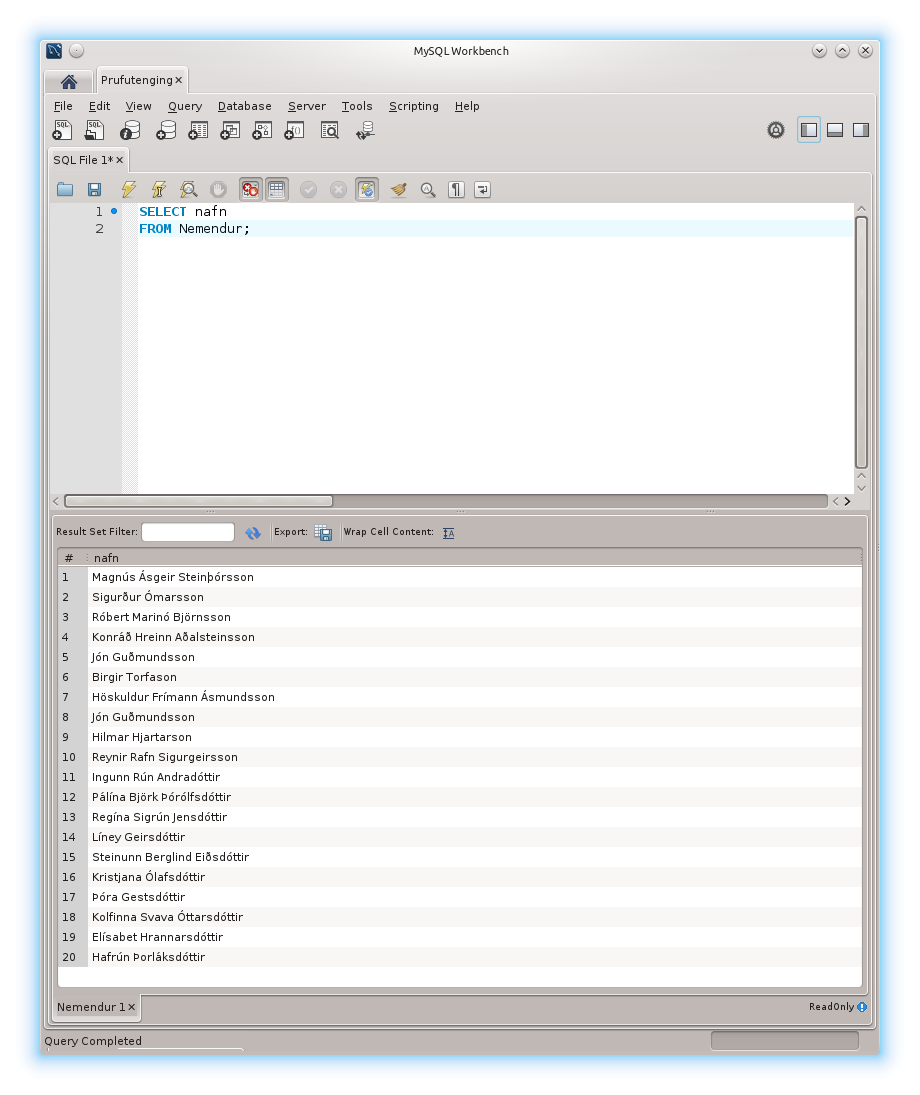
\includegraphics[width=\linewidth]{myndir/workbench-select}
\end{figure*}

\verb|SELECT| skipun getur náð í marga dálka (eða mörg atriði) í einu. Atriðin eru þá einfaldlega aðgreind með kommum. Þetta má sjá á sýnidæmi \ref{sql:k4d3-margir-dalkar}.

\begin{example}
\caption[SELECT með mörgum dálkum]{\emph{SELECT} skipun sem nær í marga dálka. }
\label{sql:k4d3-margir-dalkar}
\centering
\sql{sql/k4d3-margir-dalkar.sql}
\end{example}

\begin{table}
\centering
\caption[Niðurstaða margra dálka SELECT]{Niðurstaða skipunarinnar í sýnidæmi \ref{sql:k4d3-margir-dalkar} gæti litið út á þessa leið. Allar upplýsingarnar úr dálkunum ``nafn'' og ``kennitala'' voru valdar. Aðrir dálkar sjást ekki.}
\label{tafla:margir-dalkar-nidurstada}
\begin{tabular}{ll}
\toprule
nafn&kennitala\\
\midrule
Magnús Ásgeir Steinþórsson&090698-6489\\
Sigurður Ómarsson&251198-1369\\
Róbert Marinó Björnsson&060998-2489\\
Konráð Hreinn Aðalsteinsson&120498-8869\\
Kári Jensson&230598-2159\\
Birgir Torfason&170798-7249\\
Höskuldur Frímann Ásmundsson&020298-4139\\
Styrmir Hreinsson&210498-7889\\
Hilmar Hjartarson&020798-4599\\
Reynir Rafn Sigurgeirsson&211298-7239\\
Ingunn Rún Andradóttir&161298-1589\\
Pálína Björk Þórólfsdóttir&030798-0829\\
Regína Sigrún Jensdóttir&140798-6499\\
Líney Geirsdóttir&111098-3289\\
Steinunn Berglind Eiðsdóttir&190398-1889\\
Kristjana Ólafsdóttir&230298-4759\\
Þóra Gestsdóttir&010498-8489\\
Kolfinna Svava Óttarsdóttir&210498-5759\\
Elísabet Hrannarsdóttir&050298-3109\\
Hafrún Þorláksdóttir&250498-2849\\
\bottomrule
\end{tabular}
\end{table}

\begin{figure*}
\caption[Niðurstöður margra dálka SELECT í Workbench]{Hér sést hvernig sýnidæmi \ref{sql:k4d3-margir-dalkar} og niðurstaða \emph{SELECT} skipunarinnar sem í því er (tafla \ref{tafla:margir-dalkar-nidurstada}) getur litið út í MySQL Workbench.}
\label{mynd:workbench-nidurstada-margir-dalkar}
\centering
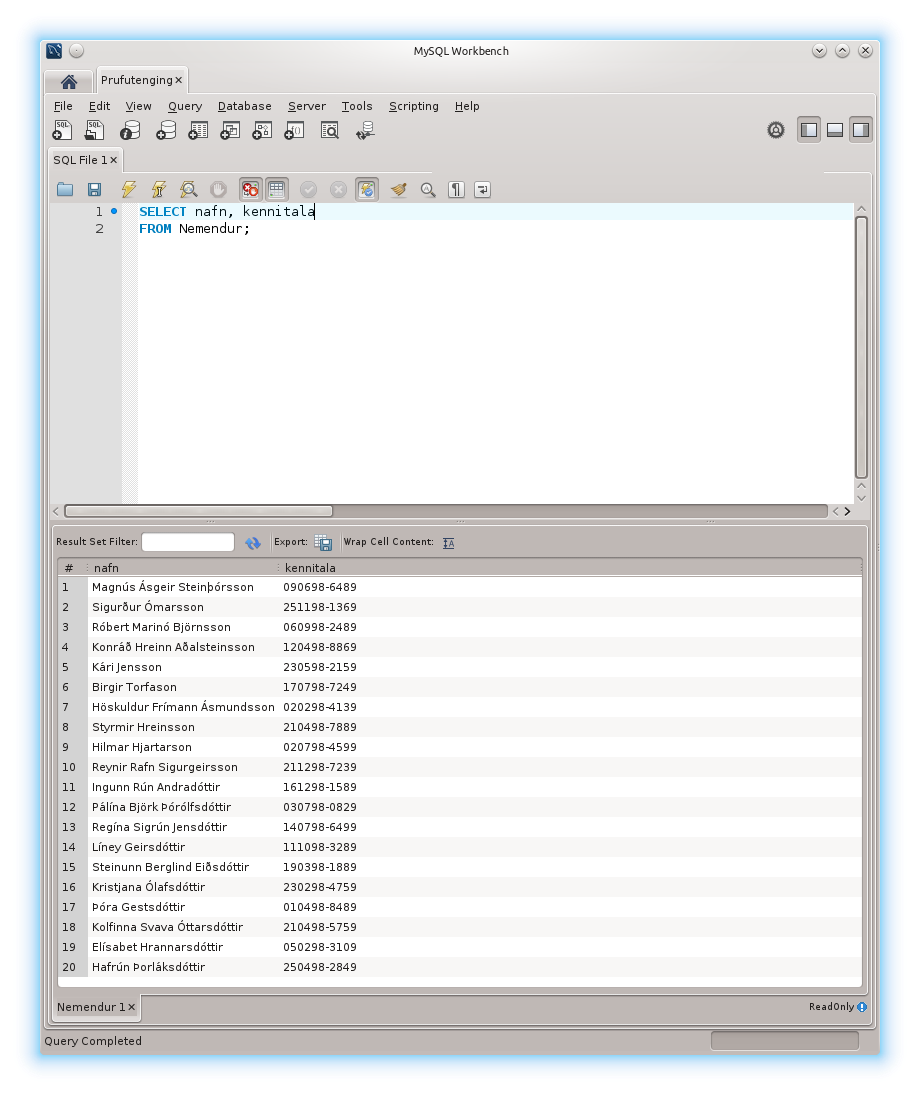
\includegraphics[width=\linewidth]{myndir/workbench-nidurstada-margir-dalkar}
\end{figure*}
\section{WHERE klausan}
Hingað til höfum við valið heila dálka með \verb|SELECT| skipunum. Það sem við viljum hins vegar oftast gera er að finna ákveðnar upplýsingar í töflunni, frekar en að fá þær allar.

Til þess að fá bara þær upplýsingar sem við viljum búum við til ``síu'' sem hleypir engum upplýsingum í gegn nema þeim sem við viljum.

Slík sía þarf að innihalda lýsingu á þeim gögnum sem hleypa á í gegn. Það er gert í klausu sem við köllum \verb|WHERE| klausu og kemur fyrir aftan \verb|FROM| klausuna. Dæmi um þetta má sjá í sýnidæmum \ref{sql:k4d4-where-numer} til \ref{mynd:workbench-nidurstada-jon}.

\begin{example}
\caption[SELECT með WHERE klausu - eftir númeri]{\emph{SELECT} skipun með \emph{WHERE} klausu sem nær í nafn nemanda (úr töflu \ref{tafla:nemendur}) þar sem ``numer'' dálkurinn er með gildið 11. Hún skilar einni línu, nafninu Ingunn Rún Andradóttir.}
\label{sql:k4d4-where-numer}
\centering
\sql{sql/k4d4-where-numer.sql}
\end{example}

\begin{example}
\caption[SELECT með WHERE klausu - eftir nafni]{\emph{SELECT} skipun með \emph{WHERE} klausu sem nær í kennitölu nemanda eftir nafni hans. Hún skilar einni línu, kennitölunni 251198-1369.}
\label{sql:k4d5-where-nafn}
\centering
\sql{sql/k4d5-where-nafn.sql}
\end{example}

\begin{example}
\caption[SELECT með WHERE klausu - endurtekin gildi]{Skilyrðið sem sett er fram í \emph{WHERE} klausu getur átt við meira en eina línu í töflunni. Þessi skipun finnur nöfn og kennitölu allra sem heita Jón Guðmundsson. Þeir reynast vera tveir, með kennitölurnar 230598-2159 og 210498-7889.}
\label{sql:k4d6-where-nafn-endurtekid}
\centering
\sql{sql/k4d6-where-nafn-endurtekid.sql}
\end{example}

\begin{figure*}[h]
\caption[Niðurstöður margra dálka SELECT í Workbench]{Hér sést sýnidæmi \ref{sql:k4d6-where-nafn-endurtekid} í MySQL Workbench.}
\label{mynd:workbench-nidurstada-jon}
\centering
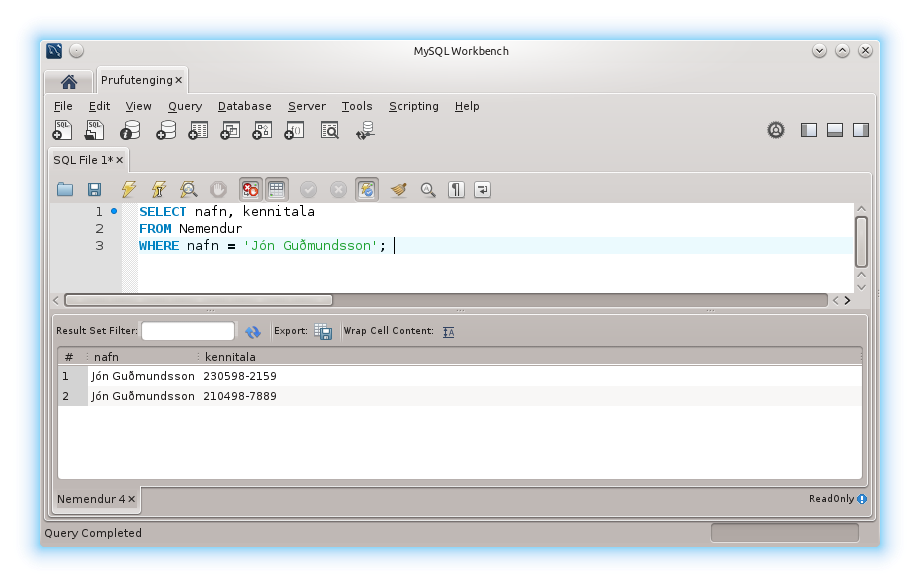
\includegraphics[width=\linewidth]{myndir/workbench-nidurstada-jon}
\end{figure*}
\subsection{Röksegðir}
Í öllum \verb|WHERE| klausunum hér á undan er um að ræða síur sem henda öllu sem ekki uppfylla eitt, nákvæmt skilyrði. Skilyrðið í sýnidæmi \ref{sql:k4d4-where-numer}, \verb|numer = 11|, hleypir til dæmis einungis þeim nemanda sem er með nákvæmlega númerið 11 í gegn.

Skilyrðin geta þó verið margs konar. \verb|WHERE| klausan tekur nefnilega við næstum hvaða röksegð\footnote{e. \emph{boolean expression}} sem er, þ.e.a.s. alls kyns samanburðum og staðhæfingum sem að lokum gefa gildin ``satt'' eða ``ósatt''.

Orðið ``röksegð'' kann að hljóma undarlega, en um kunnuglegt fyrirbæri er að ræða. ``Skilyrðið'' \verb|numer = 11| er til dæmis röksegð. Segðin er sönn þegar \verb|numer| tekur gildið 11, annars ekki. Fleiri dæmi um segðir má sjá á töflu \ref{tafla:samanburdir}.

\begin{table}
\centering
\caption[Röksegðir]{Röksegðir sem nota mætti í \emph{WHERE} klausu \emph{SELECT} skipunar. Hér er \emph{numer} nafnið á dálki sem inniheldur tölur.}
\label{tafla:samanburdir}
\begin{tabular}{ll}
\toprule
Segð&Útskýring\\
\midrule
\emph{numer} = 5&Sönn þegar gildið í \emph{numer} er nákvæmlega 5.\\
\emph{numer} > 5&Sönn þegar gildið í \emph{numer} er stærra en 5.\\
\emph{numer} < 5&Sönn þegar gildið í \emph{numer} er minna en 5.\\
\emph{numer} >= 5&Sönn þegar gildið í \emph{numer} er 5 eða stærra.\\
\emph{numer} <= 5&Sönn þegar gildið í \emph{numer} er 5 eða minna.\\
\emph{numer} != 5&Sönn þegar gildið í \emph{numer} er ekki 5.\\
\bottomrule
\end{tabular}
\end{table}

Þegar dálkheiti eru notuð í \verb|WHERE| klausu má því líta á það sem svo að við skoðum öll gildi sem eru í dálkinum, eitt í einu\footnote{Reyndar getur gagnagrunnskerfi oft gert mun betur en svo að þurfa að skoða öll gildin. Þetta tengist sérstaklega \emph{lyklum}, sem við lítum á í undirkafla \ref{undirkafli:lyklar}.}, skiptum dálkheitinu út fyrir gildið og athugum hvort að segðin sé sönn. Ef segðin sem fæst út línu í gagnagrunninum er sönn, þá fær línan að fara áfram í niðurstöðurnar. Dæmi um hvernig flokkun af þessu tagi fer fram má sjá á mynd \ref{mynd:roksegd}.

\begin{figure}
\caption[Röksegð í WHERE klausu]{Röksegð í WHERE klausu.}
\label{mynd:roksegd}
\centering
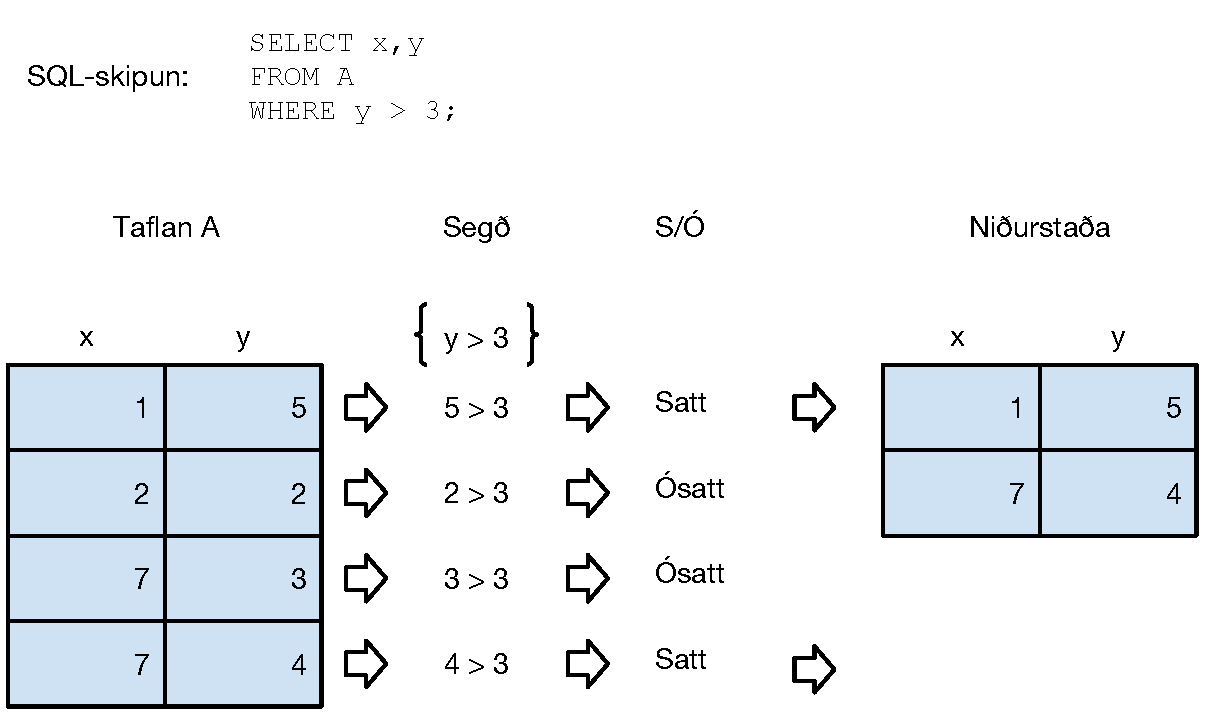
\includegraphics[width=\linewidth]{myndir/roksegd}
\end{figure}

Eins og við höfum t.d. séð á sýnidæmi \ref{sql:k4d6-where-nafn-endurtekid} þarf röksegð ekki að innihalda eingöngu samanburði með tölum. T.d. er hægt að bera saman strengi og dagsetningar.

Dagsetningar eru bornar saman líkt og tölur. Strengir eru hins vegar bornir saman í stafrófsröð. Dæmi um segðir sem innihalda strengi má sjá á töflu \ref{tafla:samanburdir-strengir}.

Nokkur atriði ber þó að varast þegar strengir eru notaðir til samanburðar í MySQL.

\newthought{Sérstakir stafir og tákn} á borð við upphrópunarmerki og bil eru ekki alltaf borin saman á þann hátt sem við giskum á. Stafrófsröð er ekki skilgreind fyrir þessi tákn. Pössum okkur þegar við notum $>$ eða $<$ til að bera saman strengi sem ekki innihalda bókstafi eingöngu.\footnote{Gagnlegt getur verið að lesa sér til um \emph{Collations} í MySQL til að öðlast frekari skilning á strengjasamanburðum. Ekki er fjallað um það í þessari bók.}

\newthought{Séu strengir af mismunandi lengdum bornir saman} er bilum bætt við hægra megin við styttri strenginn áður en samanburðurinn er framkvæmdur. Þannig myndi \verb|'a' > 'aa'| vera breytt í \verb|'a ' > 'aa'|. Þetta getur leitt til óvæntra niðurstaðna. Dæmi um niðurstöðu sem við fyrstu sýn kann að virðast undarleg má sjá á sýnidæmi \ref{sql:k4d7-where-nafn-staerra-en}.

\begin{table}
\centering
\caption[Röksegðir með strengjum]{Dæmi um hvernig MySQL meðhöndlar röksegðir með strengjum.}
\label{tafla:samanburdir-strengir}
\begin{tabular}{ll}
\toprule
Segð&Gildi\\
\midrule
\verb|'a' = 'a'|&Satt.\\
\verb|'a' >= 'a'|&Satt.\\
\verb|'b' > 'a'|&Satt, af því að $b$ er á eftir $a$ í stafrófinu.\\
\verb|'a' > 'b'|&Ósatt, af því að $b$ er á eftir $a$ í stafrófinu.\\
\verb|'ab' > 'aa'|&Satt, af því að aftari stafir útkljá jafntefli.\\
\verb|'a b' > 'a a'|&Satt, af því að bil er sagt minna en $a$.\\
\verb|'a b' > 'aaa'|&Ósatt, af því að bil er sagt minna en $a$.\\
\verb|'ab' > 'aabbb'|&Satt, af því að í samanburði mislangra strengja\\
&er bilum bætt við hægra megin við styttri strenginn.\\
\bottomrule
\end{tabular}
\end{table}

\begin{example}
\caption[Stærra-en samanburður við streng]{\emph{SELECT}-skipun sem ber saman öll nöfn við strenginn \emph{'M'}. Skipunin skilar nöfnum allra nemanda sem eru á eftir \emph{M} í stafrófinu, \emph{að nemendum sem byrja á M meðtöldum!} Þetta er vegna þess að strengurinn \emph{M} er lengdur með bilum áður en samanburðurinn er framkvæmdur. Bil er álitið ``minna'' en allir bókstafir, svo segðin verður sönn fyrir öll nöfn sem byrja á \emph{M}.}
\label{sql:k4d7-where-nafn-staerra-en}
\centering
\sql{sql/k4d7-where-nafn-staerra-en.sql}
\end{example}

\subsection{LIKE og ``wildcards''}
Táknin sem við höfum séð í \verb|WHERE| klausum (t.d. $=$ og $>$) hafa gert okkur kleift að skrifa margar mismunandi röksegðir.

Ein gerð af segð sem við höfum ekki getað gert er að athuga hvort að strengur passi við hluta af öðrum streng. Til þess höfum við ákveðið lykilorð sem heitir \verb|LIKE|.

Það að nota \verb|LIKE| í röksegð er líkt og að nota \verb|=|. \verb|LIKE| hefur þó ákveðinn möguleika sem \verb|=| hefur ekki - þann að skilja eftir ``óþekkta'' stafi í strengnum sem notaður er til samanburðar. Þessi óvissutákn geta komið í stað hvaða stafs sem er. Þau eru kölluð ``wildcards'' á ensku. Við skoðum tvö mismunandi wildcards í þessum undirkafla. 

Annars vegar er táknið \verb|_| (strik niðri). \verb|_| getur komið í staðinn fyrir hvaða \emph{einn} staf sem er í strengnum.

Hins vegar er táknið \verb|%| (prósentumerki). \verb|%| getur komið í staðinn fyrir hvaða fjölda stafa sem er.

Dæmi \ref{sql:k4d8-like-upphaf} til \ref{sql:k4d12-like-kennitala} sýna notkun \verb|LIKE| og wildcard-tákna.

\begin{example}
\caption[LIKE til að finna orð sem byrja á sama staf]{\emph{SELECT} skipun sem finnur alla nemendur í nemendatöflunni sem byrja á stafnum \emph{K}. Til þess er notaður samanburðarstrengur sem hefur wildcard-táknið \emph{\%} á eftir stafnum \emph{K}, svo að \emph{\%} komi í staðinn fyrir allt sem á eftir \emph{K} kemur.}
\label{sql:k4d8-like-upphaf}
\centering
\sql{sql/k4d8-like-upphaf.sql}
\end{example}

\begin{example}
\caption[LIKE til að finna orð sem enda eins]{\emph{SELECT} skipun sem finnur alla nemendur í nemendatöflunni sem enda á \emph{``dóttir''}. \emph{\%} kemur hér á undan \emph{``dóttir''} svo að það geti komið í staðinn fyrir alla stafi sem gætu verið þar á undan.}
\label{sql:k4d9-like-lok}
\centering
\sql{sql/k4d9-like-lok.sql}
\end{example}

\begin{example}
\caption[LIKE einhvers staðar í streng]{\emph{SELECT} skipun sem finnur alla nemendur í nemendatöflunni sem innihalda strenginn ``geir'' einhvers staðar í nafni sínu. Segðin í \emph{WHERE}-klausunni er t.d. sönn fyrir nemandann sem heitir Ásgeir að millinafni og nemandann sem er Sigurgeirsson.}
\label{sql:k4d10-like-midja}
\centering
\sql{sql/k4d10-like-midja.sql}
\end{example}

\begin{example}
\caption[LIKE til að finna strengi af ákveðinni lengd]{\emph{SELECT} skipun sem finnur alla nemendur sem eru með nákvæmlega 17 stafi í nafni sínu (að bilum meðtöldum). Hvert \_ tákn kemur í stað nákvæmlega eins stafs. Við sjáum aðra leið til að gera þetta í undirkafla \ref{undirkafli:einindafoll}.}
\label{sql:k4d11-like-nakvaemt}
\centering
\sql{sql/k4d11-like-nakvaemt.sql}
\end{example}

\begin{example}
\caption[LIKE með nákvæmum stafafjölda]{\emph{SELECT} skipun sem finnur alla nemendur í nemendatöflunni sem fæddir eru í apríl (með stafina 04 í þriðja og fjórða sæti í kennitölu sinni). Hún finnur einungis þá nemendur, vegna þess að \_ táknin tvö geta komið í staðinn fyrir nákvæmlega tvö önnur tákn, hvorki fleiri né færri.}
\label{sql:k4d12-like-kennitala}
\centering
\sql{sql/k4d12-like-kennitala.sql}
\end{example}
\subsection{Mörg aðskilin skilyrði} % AND, OR, IN

\section{Helstu einindaföll}
\label{undirkafli:einindafoll}
\subsection{LENGTH}
\subsection{ROUND}
\subsection{UCASE og LCASE}
\section{GROUP BY}
\section{Helstu samsteypuföll}
\subsection{SUM og AVG}
\subsection{MIN og MAX}
\subsection{COUNT}
\section{HAVING}
\section{ORDER BY}
\subsection{LIMIT}
\section{Yfirlit}
\subsection{Uppbygging SELECT skipunarinnar}